\documentclass[14pt]{beamer}
\usetheme{Madrid}
\usepackage[utf8]{inputenc}
\usepackage[spanish]{babel}
\usepackage{amsmath}
\usepackage{amsfonts}
\usepackage{amssymb}
\usepackage{graphicx}
\definecolor{UBCblue}{rgb}{50, 0.1, 0.1}

\usecolortheme[named=UBCblue]{structure}

\author[Campanería, Fernández, Fuentes]
{David Campanería Cisneros\\Pablo Adrian Fuentes González\\Dayron Fernández Acosta}
\title[Aplicación   HCVet]
{HCVet: Aplicación móvil para historia clínica veterinaria.}
%\setbeamercovered{transparent} 
%\setbeamertemplate{navigation symbols}{} 
\logo{
\includegraphics[height=1cm]{Images/clean_app_icon.png}} 
\institute[UH]
{\textbf{Tutores:}\\ José Alejandro Mesejo Chiong\\ José Luis Castañeda Lorenzo} 
%\date{} 
%\subject{} 
\begin{document}

\begin{frame}
\titlepage
\end{frame}



\begin{frame}
\frametitle{Temática}
\begin{block}{Temática}
Creación de una herramienta que permita gestionar los datos clínicos históricos de la condición de salud y los servicios que han recibido animales domésticos.

\end{block}

\footnote{Dayron}
\end{frame}


\begin{frame}
\frametitle{Objetivos}
El desarrollo de la app debe tener en cuenta :
\begin{itemize}
\item Facilidad de uso
\item Almacenamiento de Datos y características de animales
\item Sistema de registro de usuarios
\item Almacenamiento de Historiales Clínicos
\item Compartimiento de Datos 

\footnote{Dayron}
\end{itemize}
\end{frame}

\begin{frame}
\frametitle{Importancia del problema}
Razones por las que son necesarias resolver el problema:
\begin{itemize}
\item Gran cantidad de datos
\item Poca agilidad del sistema actual
\item Datos difícilmente transferibles
\item Inconsistencia de los Datos
\end{itemize}
\footnote{Dayron}
\end{frame}

\begin{frame}
\frametitle{Funcionalidades de la aplicación}
\begin{itemize}
\item Creación de una mascota:
\item Eliminar mascota
\item Transferir una mascota a otro usuario de manera local.
\item Insertar nueva consulta
\item Insertar notas extras
\item Visualización
\end{itemize}
\footnote{David}
\end{frame}


\begin{frame}
\frametitle{Tecnologías utilizadas}

Tecnologías utilizadas:
\begin{itemize}
\item Flutter
\item Kotlin
\item SQLite
\end{itemize}
\footnote{David}
\end{frame}


\begin{frame}
\frametitle{Patrón Arquitectónico}

Fue utilizado un patrón \textbf{Model-View-ViewModel}.
\\
Componentes:
\begin{itemize}
\item Model
\item View
\item ViewModel
\end{itemize}

\footnote{David}
\end{frame}





\begin{frame}
\frametitle{Estructura de Model}

\begin{itemize}
\item Componente de comunicación con el servidor (Online)

\item Componente de transferencia de datos no sincronizada sin conexión a internet. (Offline)

\item Componente de almacenamiento interno (Database)

\end{itemize}

\footnote{David}
\end{frame}

\begin{frame}
\frametitle{Componente de comunicación con el servidor.}

\begin{block}{}
Se establece comunicación con el servidor a través del protocolo HTTPS.
\end{block}
\footnote{David}
\end{frame}

\begin{frame}
\frametitle{Componente de transferencia de datos offline.}

\begin{block}{}
En la implementación de este componente fue utilizado Kotlin para hacer uso del API WifiP2pManager de Android.

Las bibliotecas de Flutter para el manejo de conexiones vía Wifi entre dispositivos están restringidos para SDK de Android mayor o igual que 26.
\end{block}
\footnote{David}
\end{frame}

\begin{frame}
\frametitle{Componente de almacenamiento interno.}

\textbf{Algunos de los métodos proporcionados por el paquete sqflite para el manejo de base de datos SQLite:}

\begin{itemize}


\item execute(...)
\item insert(...)
\item update(...)
\item query(...)
\item delete(...)
\end{itemize}
\footnote{Pablo}
\end{frame}



\begin{frame}
\frametitle{Modelo de Datos}

\begin{center}

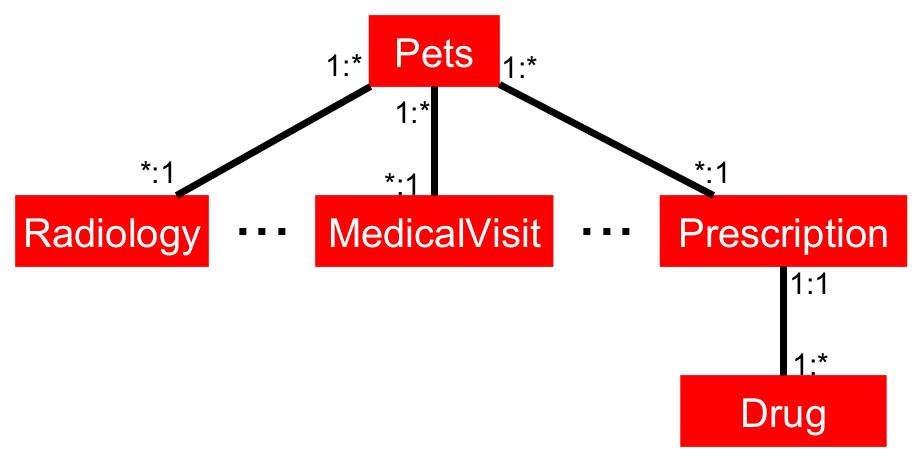
\includegraphics[scale =0.35]{Images/symplifiedClass.jpg}

\end{center}

\footnote{Pablo}
\end{frame}


\begin{frame}
\frametitle{Estructura de View}
Los 5 principios utilizados para el diseño de la interfaz:
\begin{itemize}
\item Simplicidad
\item Eficiencia
\item Consistencia
\item Retroalimentación (Feedback)
\item Accesibilidad
\end{itemize}
\footnote{Dayron}
\end{frame}

\begin{frame}
\frametitle{Estructura de View}
Las dos aproximaciones utilizadas para el diseño:

\begin{columns}
\begin{column}{0.5\textwidth}
\textbf{Menu-driven interface}
\begin{center}

\fbox{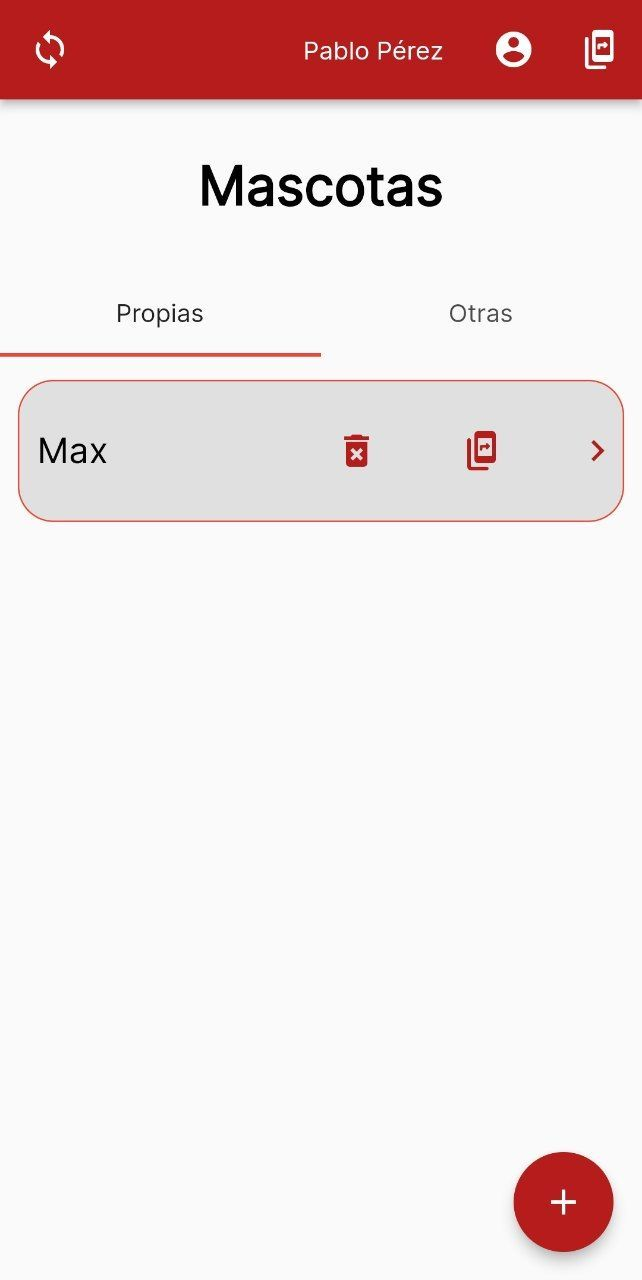
\includegraphics[scale = 0.12]{Images/homePage.jpg}}

\end{center}
\end{column}
\begin{column}{0.5\textwidth}
\textbf{Form-based interface}
\begin{center}

\fbox{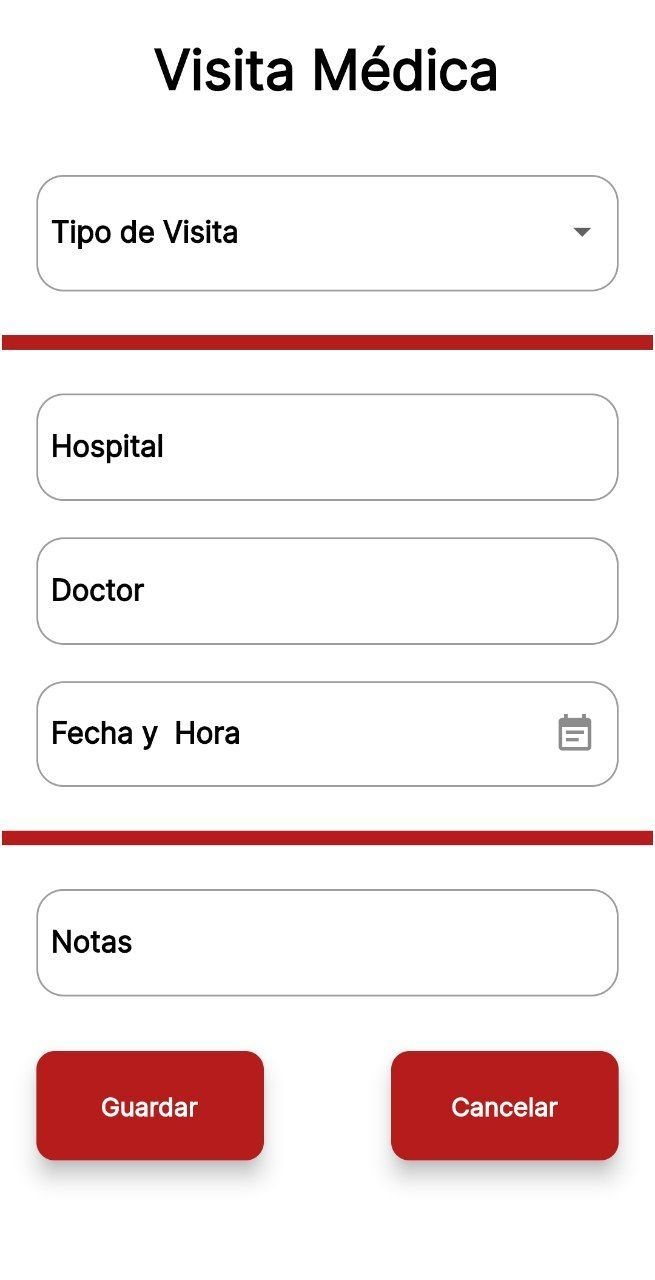
\includegraphics[scale = 0.12]{Images/form.jpg}}

\end{center}
\end{column}
\end{columns}
\footnote{Dayron}
\end{frame}


\begin{frame}
\frametitle{Estructura de View-Model}
Componentes del View-Model:
\begin{itemize}
\item SyncroVM
\item KotlinChannelVM
\item DataBaseVM


\end{itemize}

\footnote{Dayron}
\end{frame}


\begin{frame}
\frametitle{Aplicación}
\begin{columns}
\begin{column}{0.25\textwidth}
\begin{center}

\fbox{
\includegraphics[scale = 0.1]{Images/init.jpg}}
\begin{small}
\caption{Página Inicial de la Aplicación}
\end{small}
\end{center}
\end{column}

\begin{column}{0.25\textwidth}
\begin{center}

\fbox{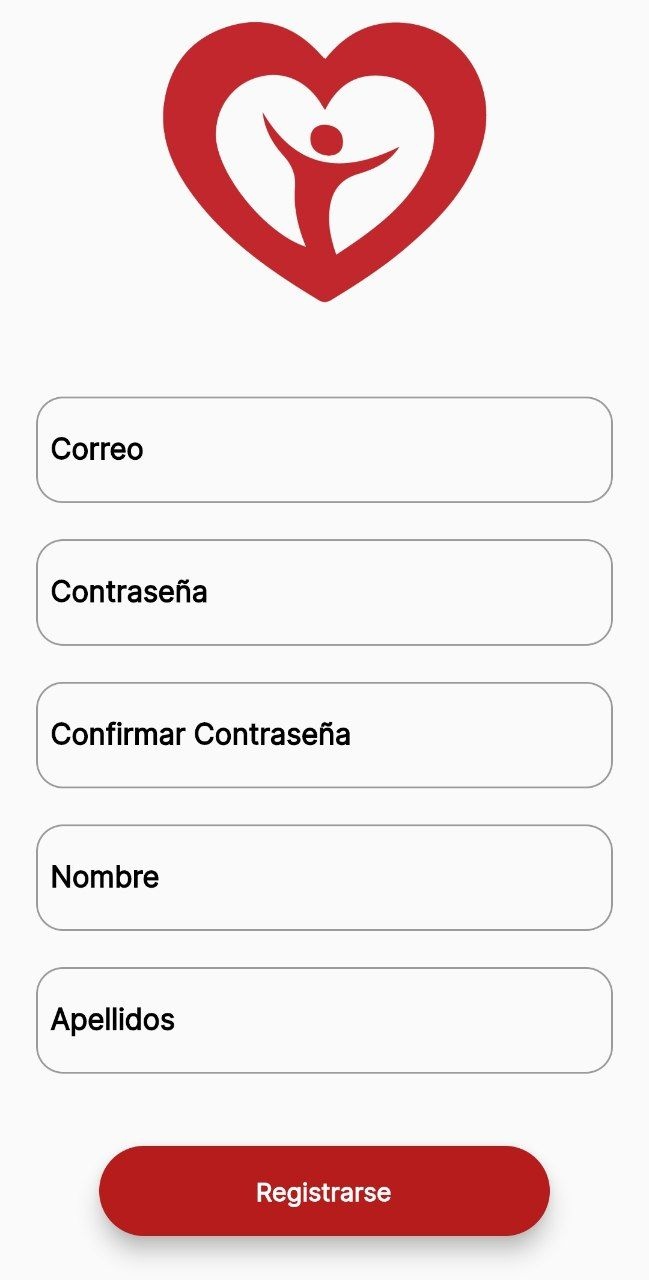
\includegraphics[scale = 0.1]{Images/register.jpg}}
\begin{small}
\caption{Página de Registro}
\end{small}
\end{center}
\end{column}

\begin{column}{0.25\textwidth}
\begin{center}

\fbox{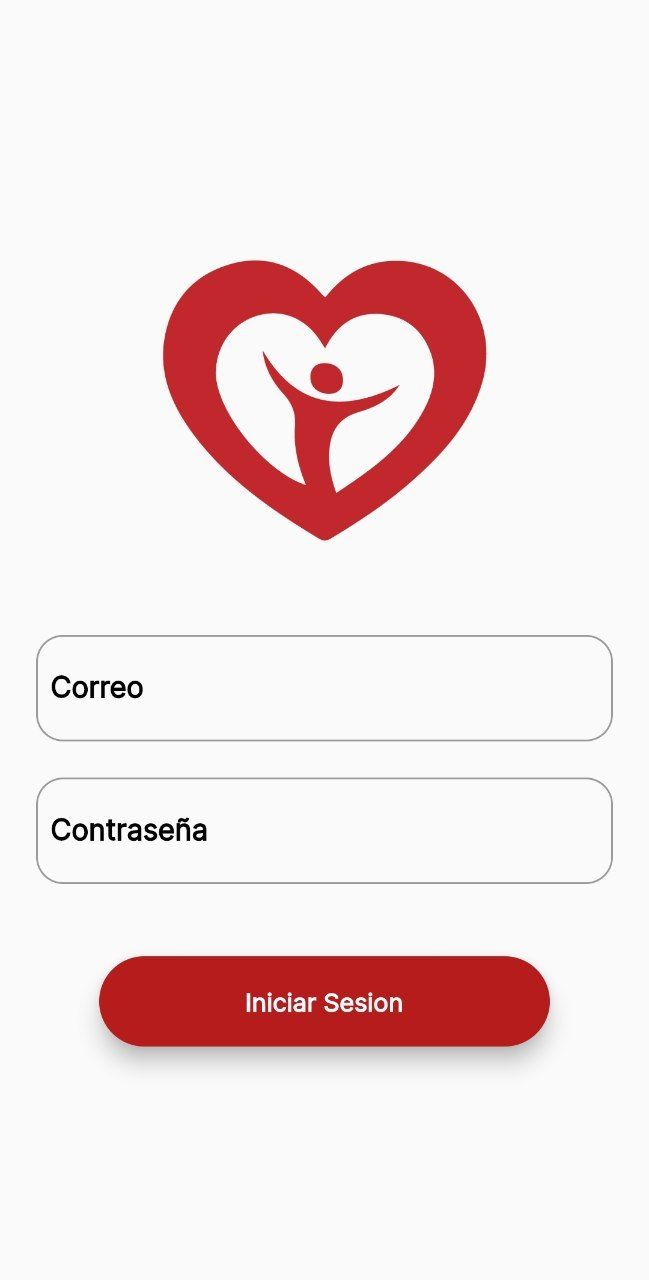
\includegraphics[scale = 0.1]{Images/login.jpg}}
\begin{small}
\caption{Página de Autenticación}
\end{small}
\end{center}
\end{column}

\end{columns}
\end{frame}




\begin{frame}
\frametitle{Aplicación}

\begin{columns}
\begin{column}{0.25\textwidth}
\begin{center}

\fbox{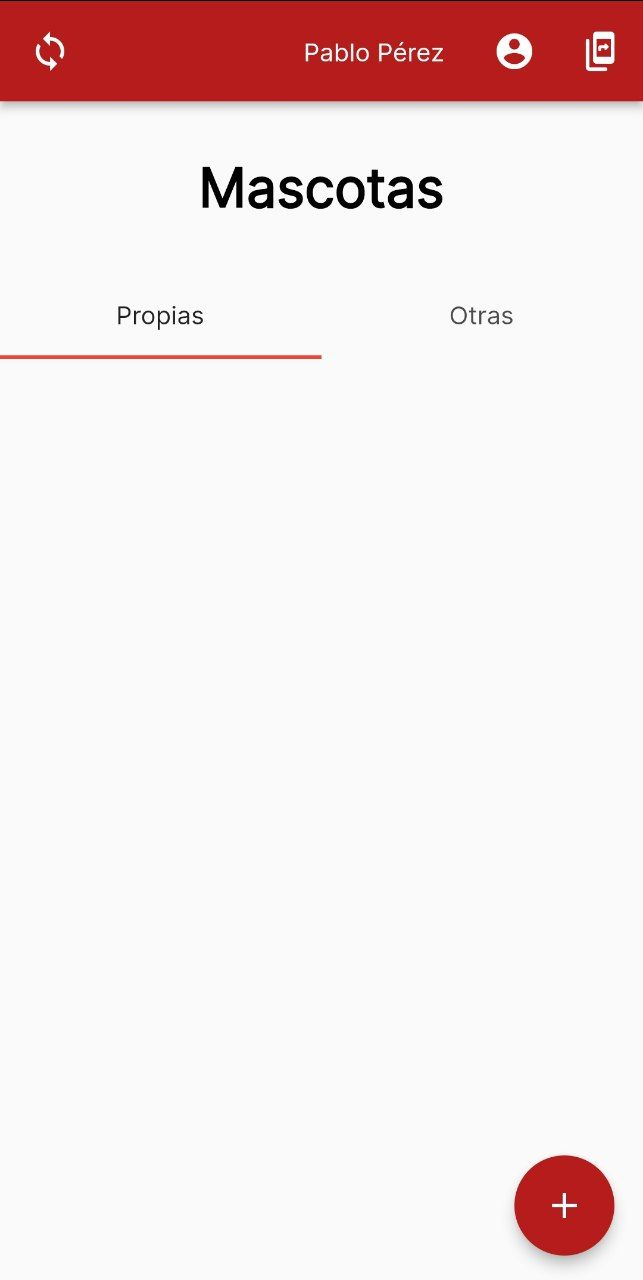
\includegraphics[scale = 0.1]{Images/home.jpg}}

\end{center}
\end{column}

\end{columns}

\end{frame}


\begin{frame}
\frametitle{Aplicación}

\begin{columns}

\begin{column}{0.5\textwidth}
\begin{center}

\fbox{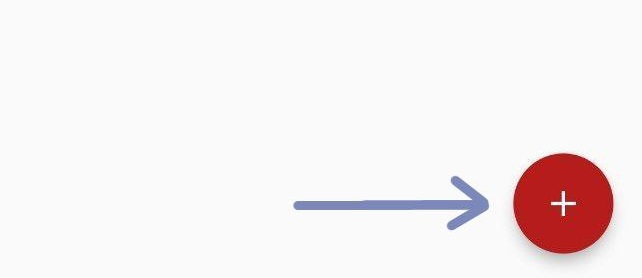
\includegraphics[scale = 0.16]{Images/createButt.jpg}}
\begin{small}


\caption{Botón de Crear Mascota}
\end{small}
\end{center}
\end{column}



\begin{column}{0.5\textwidth}
\begin{center}

\fbox{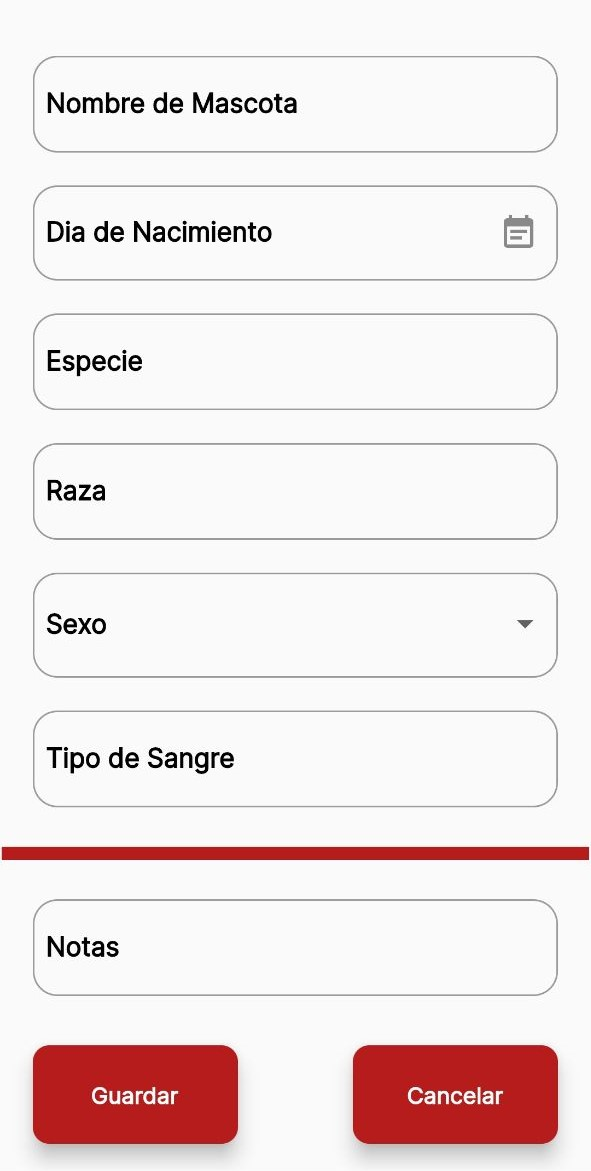
\includegraphics[scale = 0.16]{Images/createPet.jpg}}
\begin{small}



\caption{Página de Creación de Mascotas}
\end{small}
\end{center}
\end{column}

\end{columns}
\footnote{Dayron}
\end{frame}


\begin{frame}
\frametitle{Aplicación}

\begin{columns}
\begin{column}{0.25\textwidth}
\begin{center}

\fbox{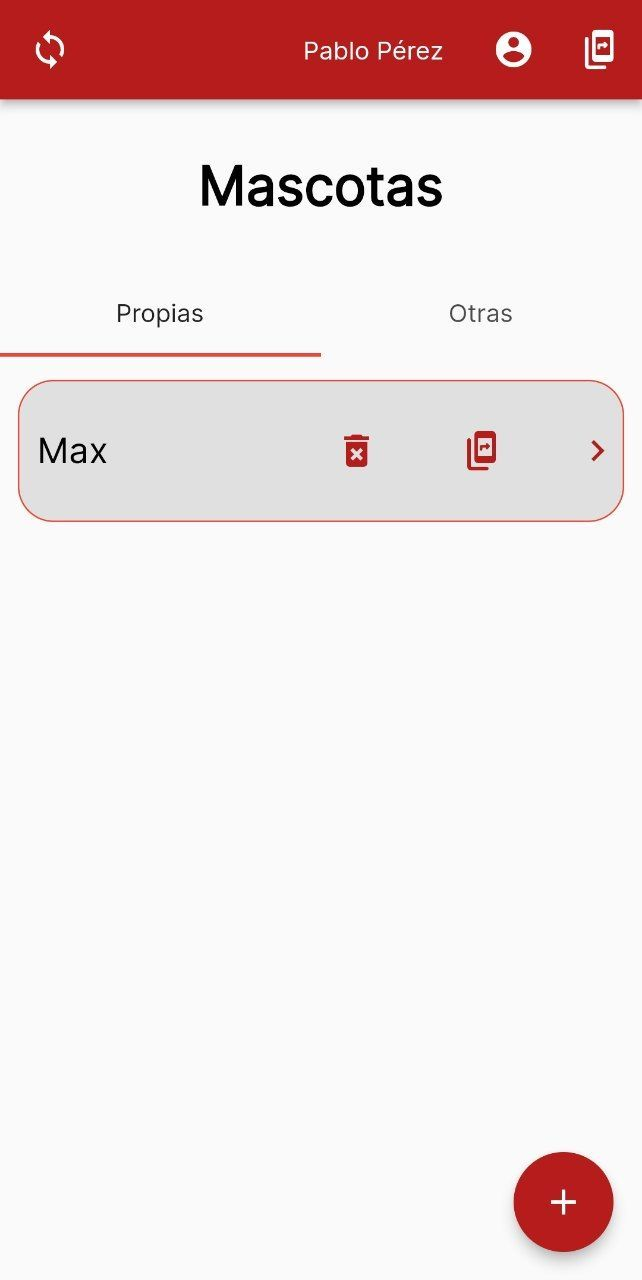
\includegraphics[scale = 0.12]{Images/homePage.jpg}}

\end{center}
\end{column}

\end{columns}
\footnote{Dayron}
\end{frame}


\begin{frame}
\frametitle{Aplicación}
Advertencia sobre la eliminación de una mascota
\begin{columns}
\begin{column}{0.25\textwidth}
\begin{center}

\fbox{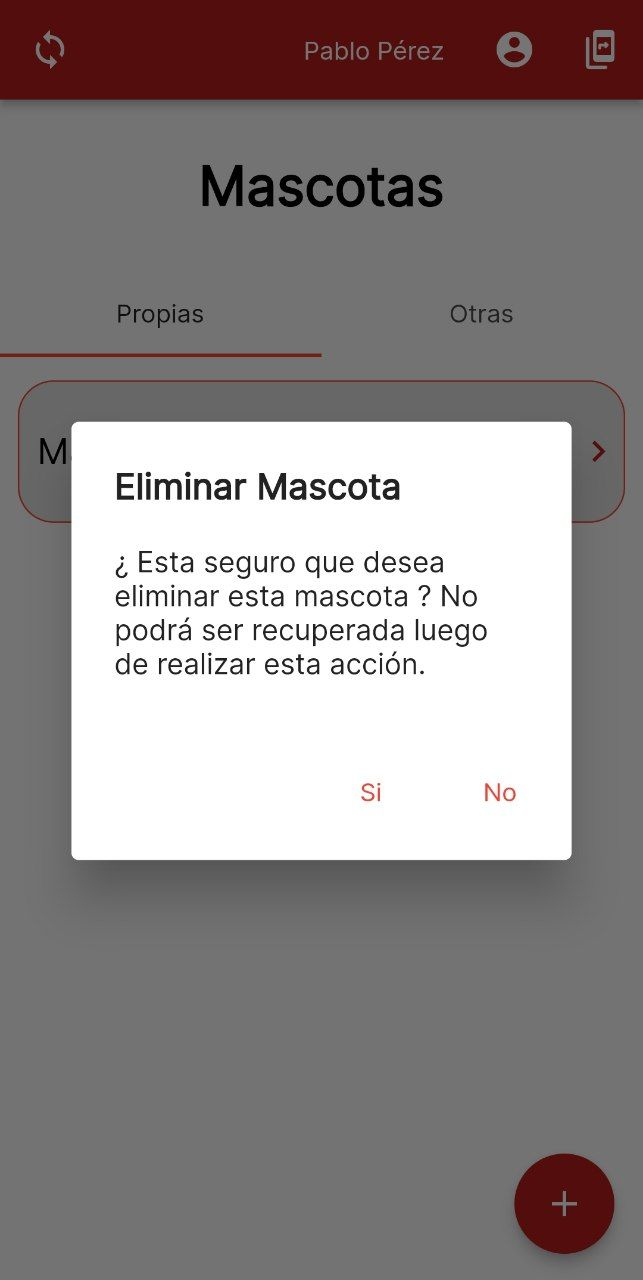
\includegraphics[scale = 0.12]{Images/deleteWarning.jpg}}

\end{center}
\end{column}

\end{columns}
\footnote{Dayron}
\end{frame}



\begin{frame}
\frametitle{Aplicación}
Botones de importación y exportación de mascota
\begin{columns}
\begin{column}{0.5\textwidth}
\begin{center}

\fbox{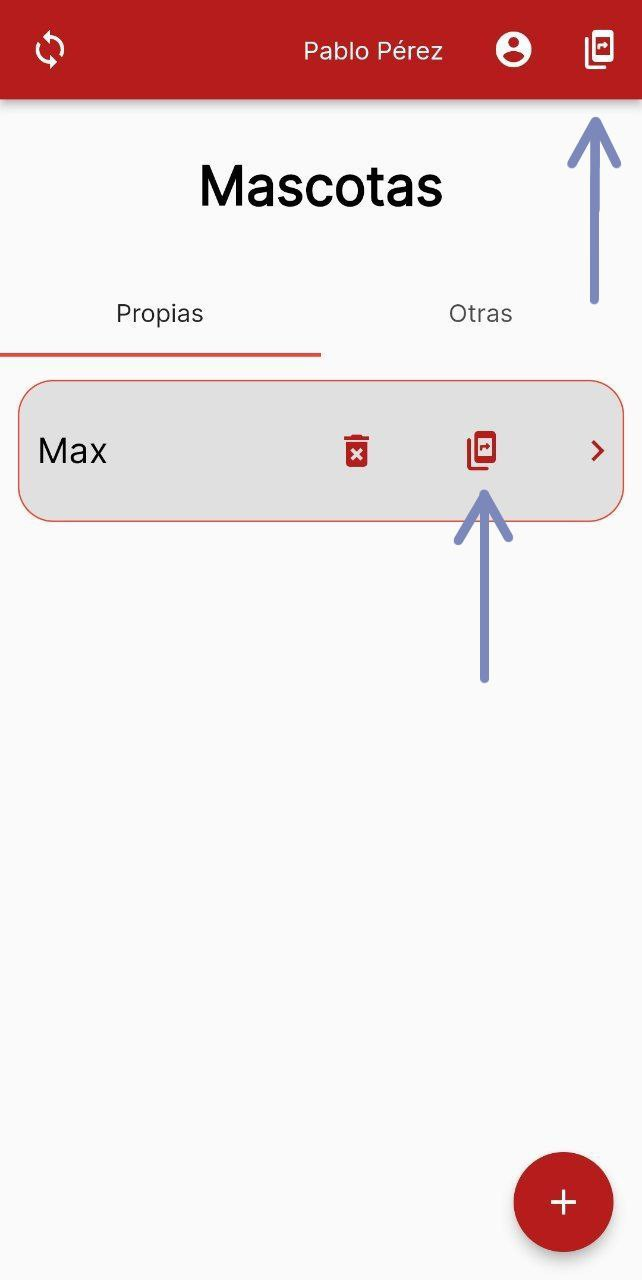
\includegraphics[scale = 0.12]{Images/homeA1.jpg}}

\end{center}
\end{column}

\end{columns}
\footnote{Dayron}
\end{frame}





\begin{frame}
\frametitle{Aplicación}
\begin{columns}
\begin{column}{0.3\textwidth}
\begin{center}

\fbox{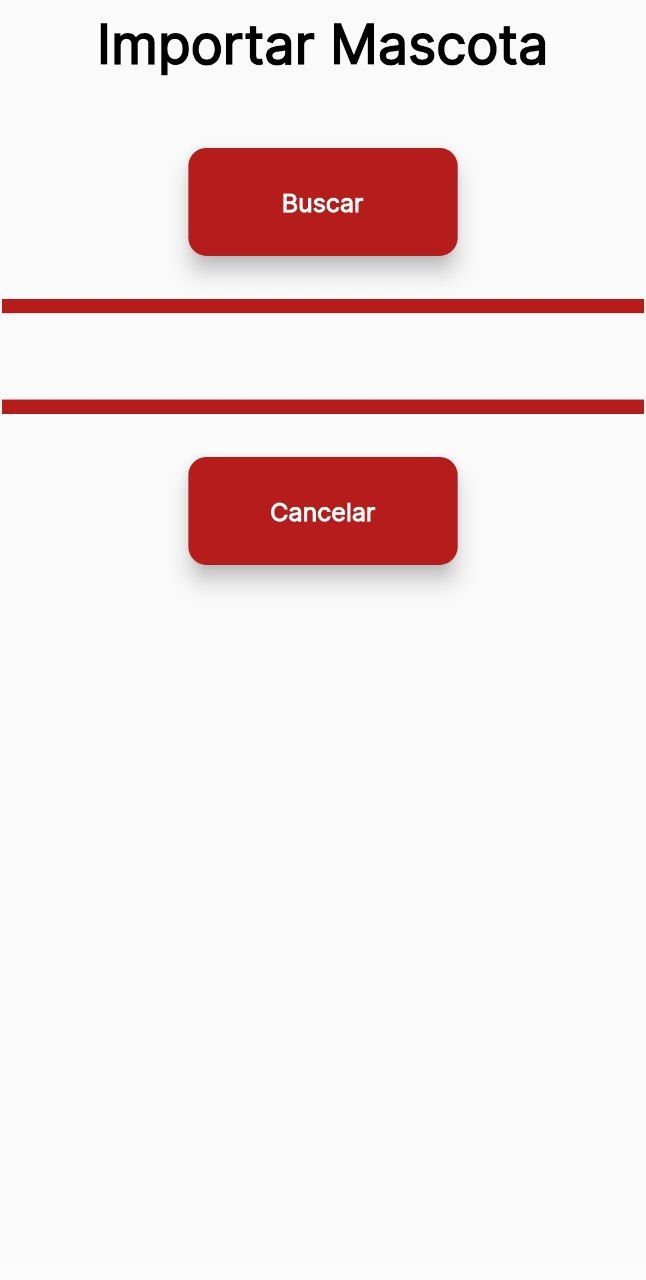
\includegraphics[scale = 0.1]{Images/import.jpg}}
\begin{small}
\caption{Página de Importación}
\end{small}
\end{center}
\end{column}

\begin{column}{0.3\textwidth}
\begin{center}

\fbox{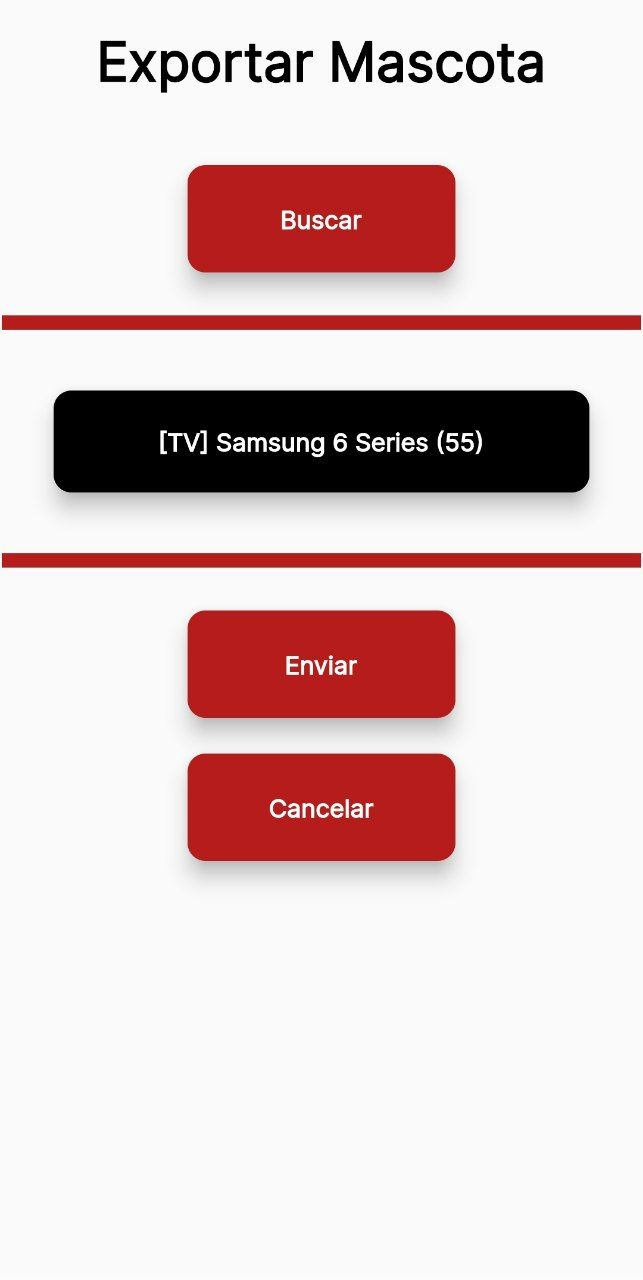
\includegraphics[scale = 0.1]{Images/exportdevice.jpg}}
\begin{small}
\caption{Página de Exportación}
\end{small}

\end{center}
\end{column}

\end{columns}
\footnote{Dayron}
\end{frame}



\begin{frame}
\frametitle{Aplicación}

\begin{columns}
\begin{column}{0.3\textwidth}
\begin{center}

\fbox{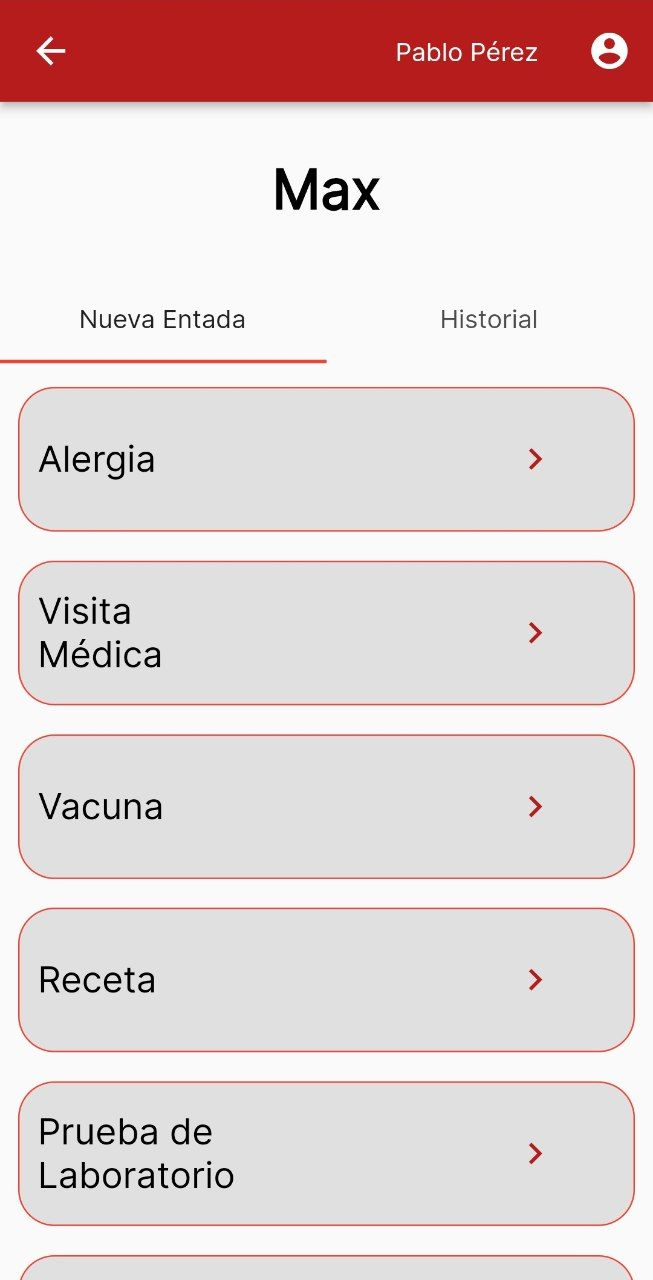
\includegraphics[scale = 0.1]{Images/addForm.jpg}}
\begin{small}
\caption{Página de Formularios}
\end{small}
\end{center}
\end{column}

\begin{column}{0.3\textwidth}
\begin{center}

\fbox{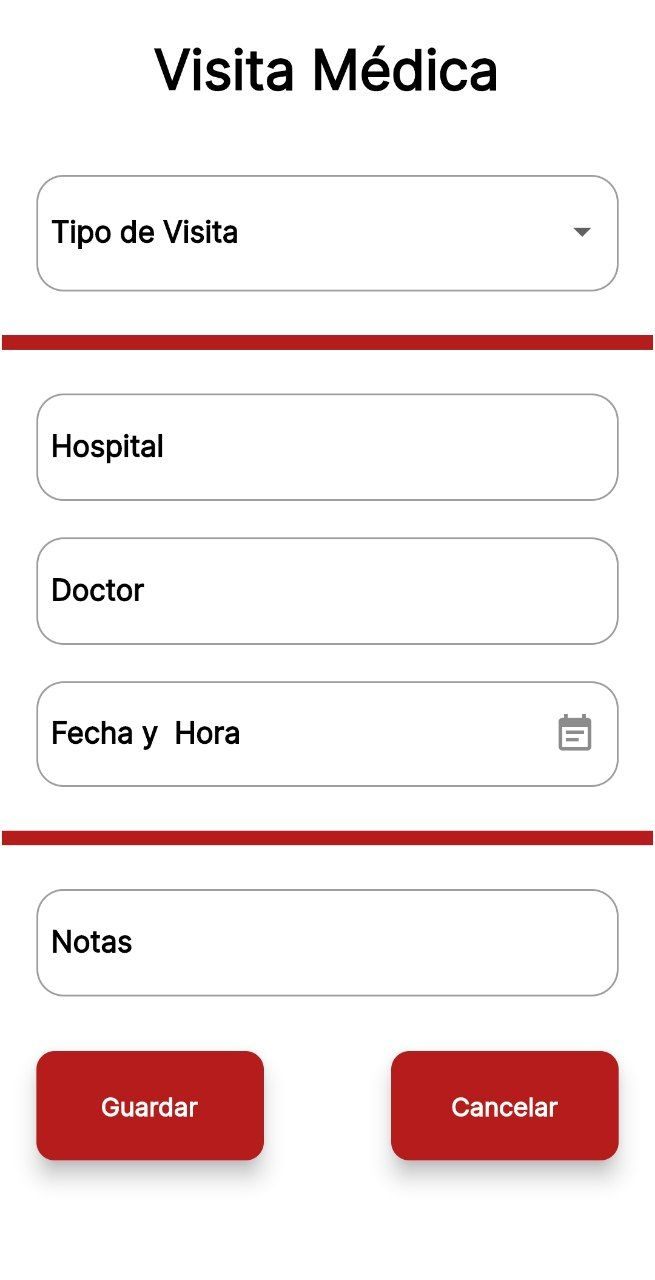
\includegraphics[scale = 0.1]{Images/MedVis.jpg}}
\begin{small}
\caption{Formulario de Visita Médica}
\end{small}
\end{center}
\end{column}

\end{columns}
\footnote{Dayron}
\end{frame}


\begin{frame}
\frametitle{Aplicación}

\begin{columns}
\begin{column}{0.3\textwidth}
\begin{center}

\fbox{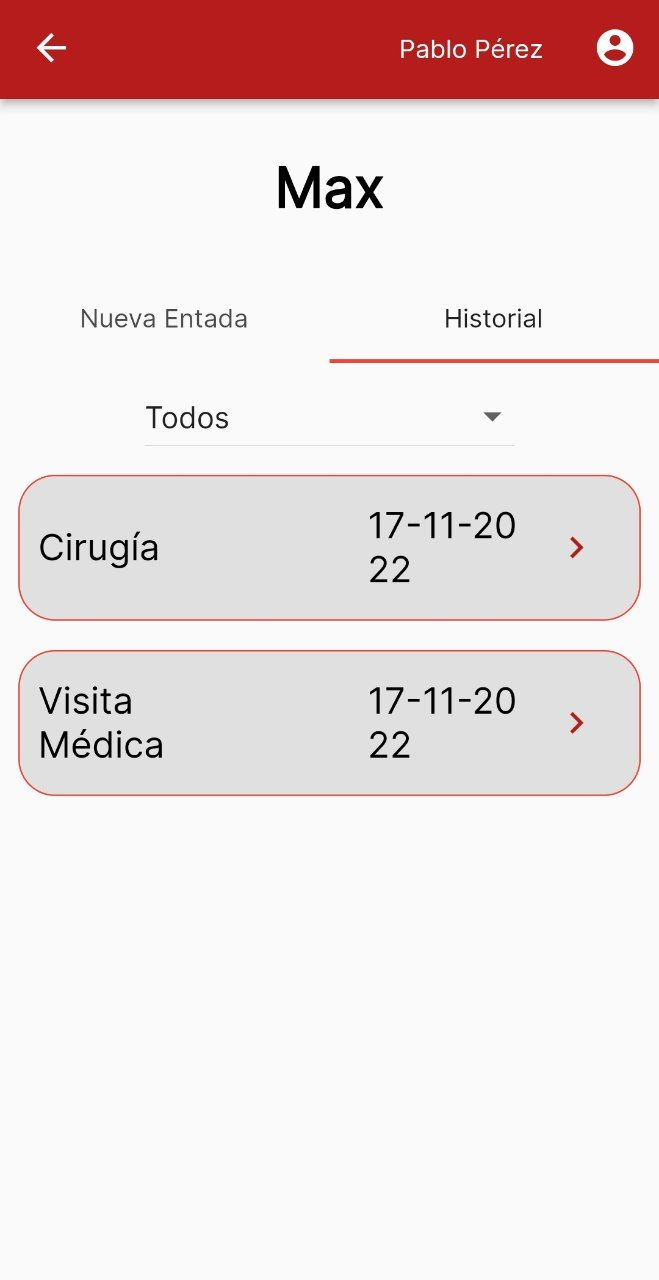
\includegraphics[scale = 0.1]{Images/hc.jpg}}

\end{center}
\end{column}

\begin{column}{0.3\textwidth}
\begin{center}

\fbox{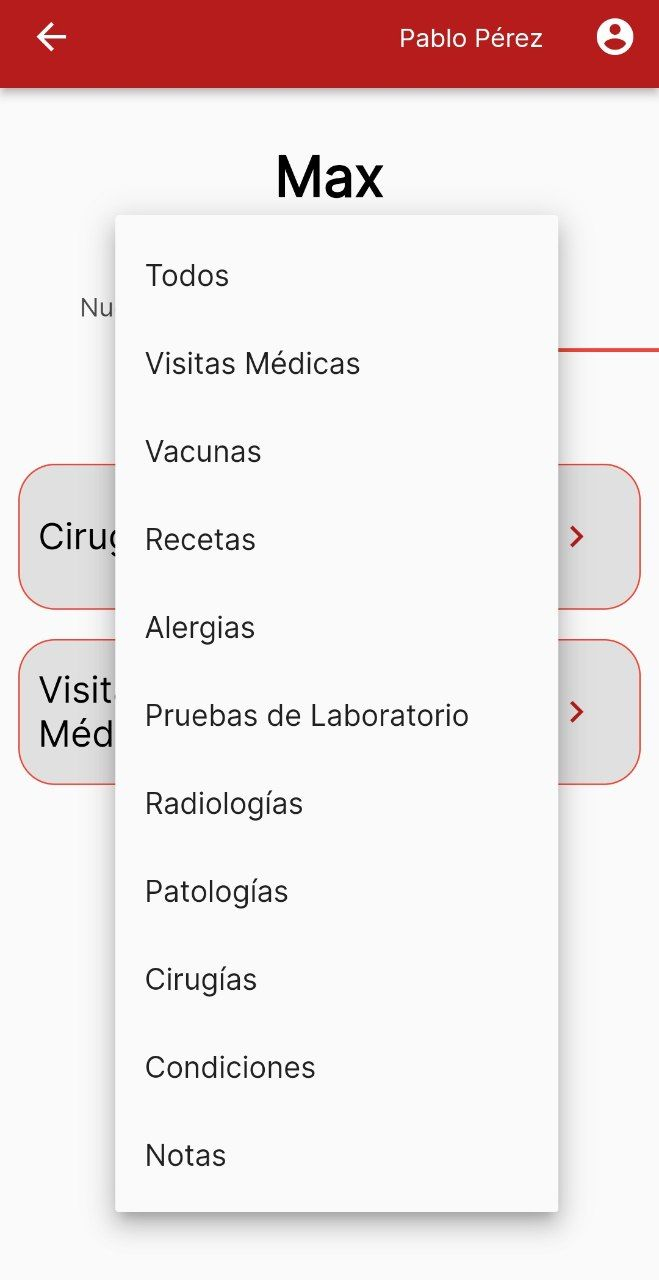
\includegraphics[scale = 0.1]{Images/selecthc.jpg}}

\end{center}
\end{column}

\end{columns}
\footnote{Dayron}
\end{frame}


\begin{frame}
\frametitle{Aplicación}

\begin{columns}
\begin{column}{0.25\textwidth}
\begin{center}

\fbox{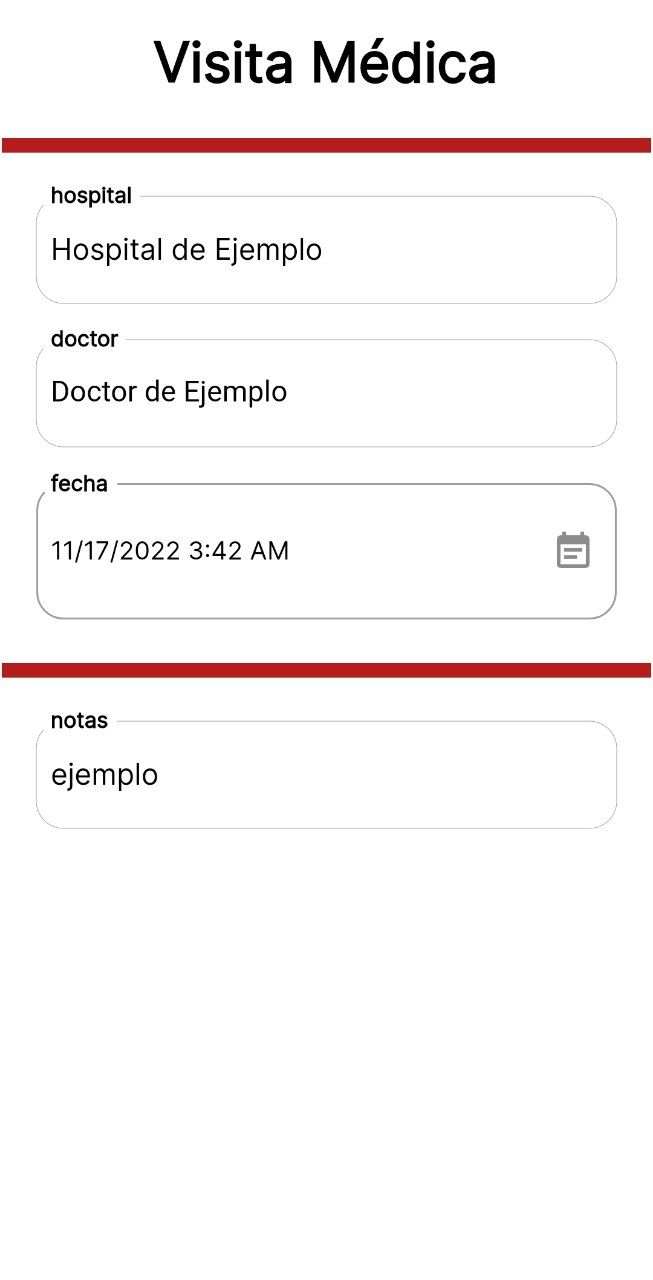
\includegraphics[scale = 0.12]{Images/medVshow.jpg}}

\end{center}
\end{column}


\end{columns}
\footnote{Dayron}
\end{frame}



\begin{frame}
\frametitle{Aplicación}

\begin{columns}

\begin{column}{0.5\textwidth}
\begin{center}

\fbox{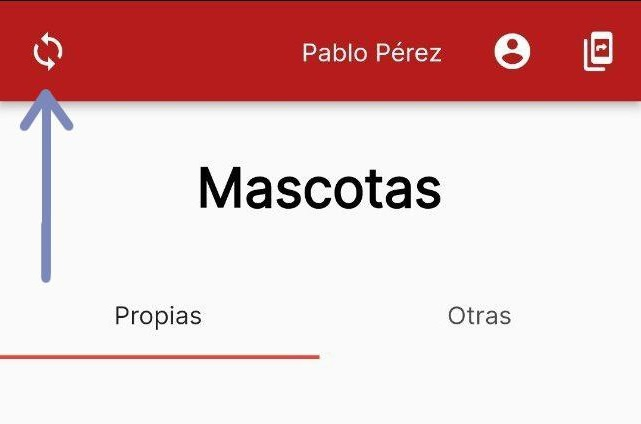
\includegraphics[scale = 0.2]{Images/synButt.jpg}}
\begin{small}
\caption{Botón de Sincronización Manual}
\end{small}
\end{center}
\end{column}


\begin{column}{0.5\textwidth}
\begin{center}

\fbox{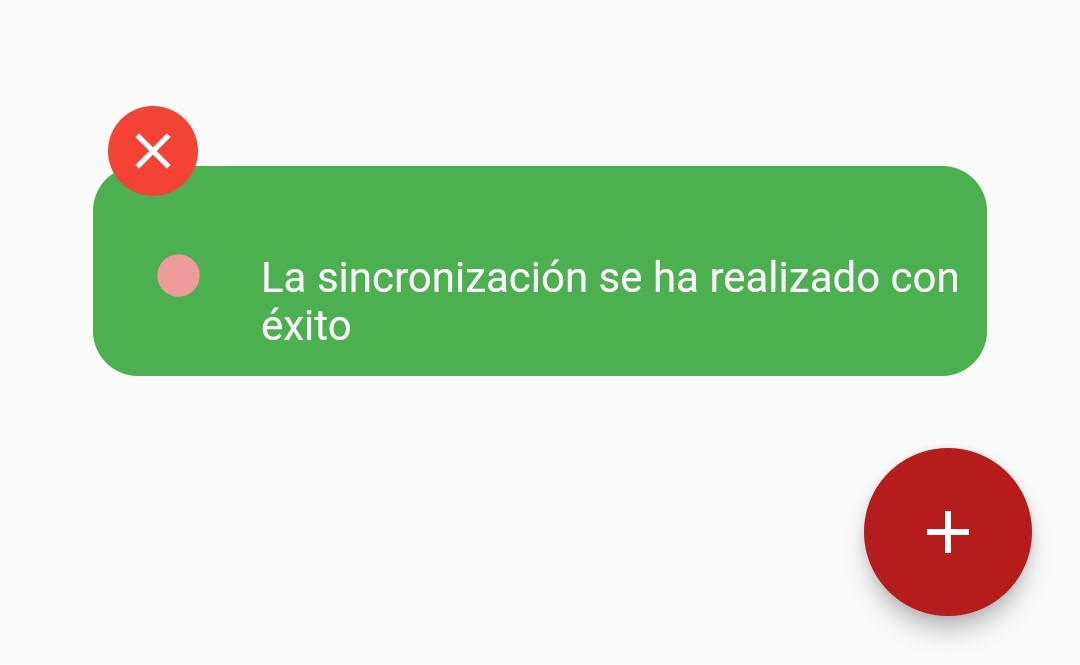
\includegraphics[scale = 0.17]{Images/synchro.jpg}}
\begin{small}
\caption{Mensaje de Sincronización Exitosa}
\end{small}
\end{center}
\end{column}


\end{columns}
\footnote{Dayron}
\end{frame}



\begin{frame}
\frametitle{Conclusiones}
\begin{itemize}
\begin{columns}
\begin{column}{0.5\textwidth}

\begin{center}

\fbox{
\includegraphics[scale = 0.12]{Images/initialPage.jpg}}

\end{center}
\end{column}
\begin{column}{0.5\textwidth}

\begin{center}

\fbox{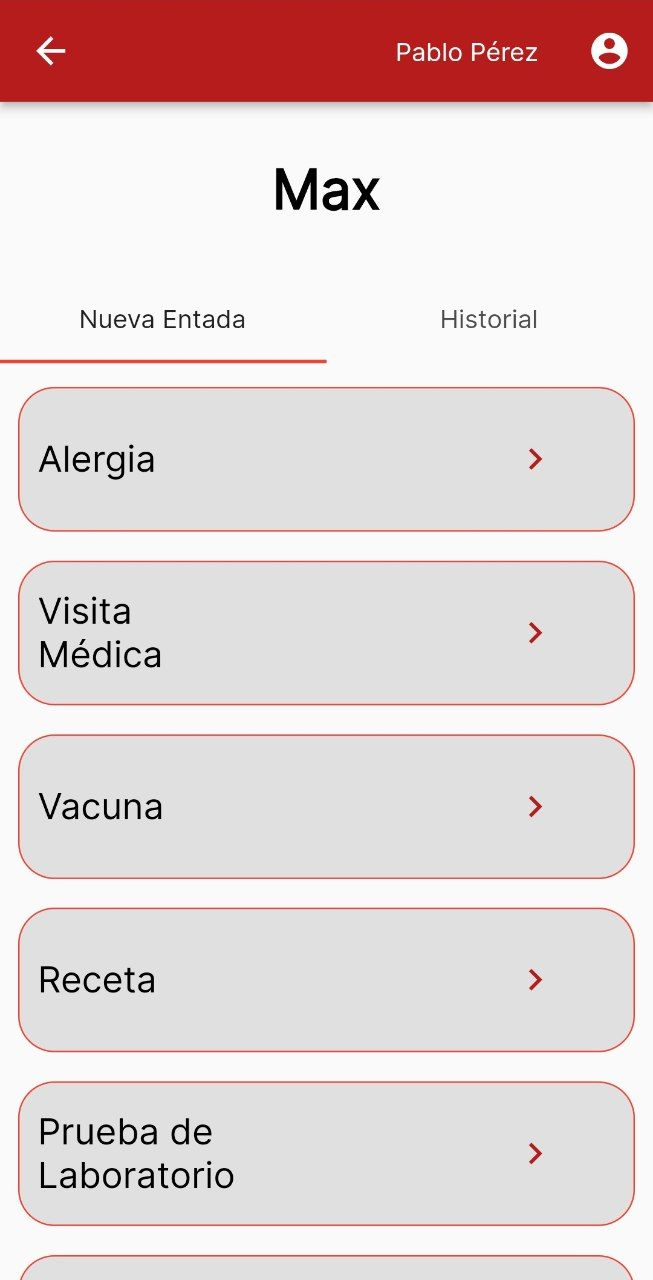
\includegraphics[scale = 0.12]{Images/pet.jpg}}

\end{center}
\end{column}
\end{columns}
\end{itemize}
\footnote{Pablo}
\end{frame}



\begin{frame}
\frametitle{Recomendaciones}

\begin{itemize}
\item Otros tipos de consultas.
\item Modificar datos.
\item Sistema de citas controlado por el servidor.
\item Diferenciar entre distintos tipos de usuarios.
\item Sistema de avisos y alarmas.
\end{itemize}

\footnote{Pablo}
\end{frame}





\begin{frame}
\maketitle
\end{frame}




\begin{frame}
\frametitle{Primera pregunta del oponente}
\begin{block}{Pregunta 1}
Aparente contradicción entre la selección de una tecnología en la hipótesis y el contenido de una de las tareas planteadas.
\end{block}
\end{frame}


\begin{frame}
\frametitle{Primera pregunta del oponente}
\begin{block}{Hipótesis}
"...sobre la plataforma Flutter a través de Dart, es posible crear un interfaz de usuario funcional..."
\end{block}

\begin{alertblock}{Tareas}
\begin{itemize}
\item ''Analizar y probar tecnologías de desarrollo de aplicaciones móviles ..."
\end{itemize}

\end{alertblock}
\end{frame}

\begin{frame}
\frametitle{Tecnologías analizadas}
\begin{itemize}
\item Java
\item Kotlin
\item Xamarin
\item React Native
\item \textbf{Flutter}

\end{itemize}

\end{frame}


\begin{frame}
\frametitle{Segunda pregunta del oponente}
\begin{block}{Pregunta 2}
¿Han considerado la idea de incluir fotos e inlcuso videos del comportamiento del animal como parte de la historia, pensando en futuras comparaciones visuales por parte de los profesionales al consultarlos?
\end{block}
\end{frame}




\begin{frame}
\frametitle{Primeros diseños de la aplicaión(7/2022)}


\begin{columns}
\begin{column}{0.5\textwidth}
\begin{center}

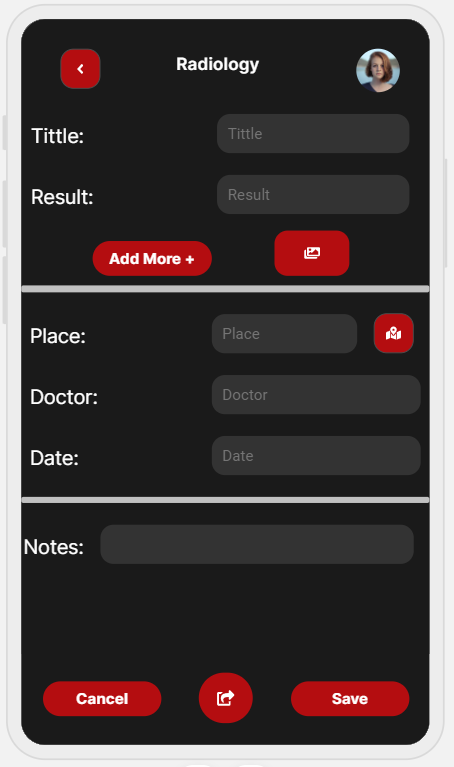
\includegraphics[scale = 0.35]{Images/photoExample.png}

\end{center}
\end{column}
\begin{column}{0.5\textwidth}
\begin{center}

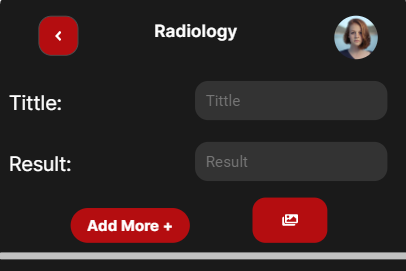
\includegraphics[scale = 0.55]{Images/photoExampleZoom.png}

\end{center}
\end{column}
\end{columns}

\end{frame}

\end{document}